\subsection{Định nghĩa hàm số và đại lượng liên quan đến hàm số}

\ % Lùi đầu dòng

Chúng ta gọi $f$ là một \emph{hàm số} (hay \emph{hàm}) đi từ tập $X$ đến tập $Y$ khi và chỉ khi với mọi $x\in X$, gọi là \emph{tập xác định}, thông qua mối liên hệ $f$ có một và chỉ một $y\in Y$ tương ứng với $x$. Câu vừa rồi có thể được tóm gọn trong một vài kí hiệu: \begin{align*}f: X &\to Y \\ x &\mapsto y.\end{align*} Khi này, chúng ta có thể viết mối liên hệ hàm số này dưới dạng biểu thức giải tích $y=f(x)$, gọi $y$ là hàm của $x$. Tuy nhiên, cần phải để ý rằng, thông qua định nghĩa này, mặc dù mọi $x$ trong $X$ phải có đầu ra trong $Y$, không phải mọi $y$ trong $Y$ đều phải có đầu vào trong $X$. Nói cách khác, tập tất cả các giá trị đầu ra có thể của $y=f(x)$, gọi là \emph{tập giá trị}, là tập con của tập $Y$.

Khi chúng ta có định nghĩa hàm số thì chúng ta cũng sẽ có những khái niệm liên quan. Khi $f$ là một hàm số, thì bất cứ giá trị $a$ thuộc tập xác định để $f(a) = 0$ đều được gọi là \emph{nghiệm} của $f$. Mở rộng ra, với $f$ và $g$ là hai hàm số, bất cứ giá trị $a$ thỏa mãn $f(a) = g(a)$ thì $a$ được gọi là nghiệm của \emph{phương trình} $f(x) = g(x)$. Hơn thế nữa, nếu thay dấu $=$ trong câu vừa trước bởi các dấu $<$, $>$, $\leq$, $\geq$, $\neq$ thì chúng ta có định nghĩa cho nghiệm của \emph{bất phương trình}. Lấy ví dụ, với $f$ và $g$ là hai hàm số, giá trị $a$ để $f(a) \neq g(a)$ thì $a$ được gọi là nghiệm của bất phương trình $f(x) \neq g(x)$\footnote{Phần lớn các tại liệu khác quên mất sự tồn tại của dấu $\neq$ rồi. Trong tài liệu này, cũng không có nhiều cơ hội để dùng dấu $\neq$ cho nên tác giả sẽ cho nó nhiều \dblquote{đất diễn} nhất có thể.}. Kết hợp nhiều phương trình hay bất phương trình, chúng ta có một \emph{hệ}. Ví dụ:
$$
\begin{cases}
   f(x) = g(x) \\
   \alpha(y) \neq \beta(z)
\end{cases}.
$$
Để thỏa mãn hệ thì mỗi thành phần trong hệ đều phải thỏa mãn.

Nếu chỉ có số với chữ không thì hàm số sẽ chở nên rất đơn điệu, cho nên người ta đã nghĩ ra phương pháp biểu diễn hàm số qua đồ thị\footnote{\dblquote{Chỉ cần}? Đương nhiên là không đơn giản như vậy. Với hàm có vô số điểm thì thông thường người ta sẽ lấy một số lượng nhất định những điểm rồi nối lại. Mà kể cả như vậy, vẫn có trường hợp không vẽ được một cách thỏa đáng. Ví dụ như hàm Đi-rích-lê: $$f(x) =
\begin{cases}
   1 \text{ nếu } x\in \mathbb{Q} \\
   0 \text{ nếu } x\notin \mathbb{Q}
\end{cases}$$ với $\mathbb{Q}$ là tập số hữu tỉ. Những hàm như thế này đã mang đến nhiều sự đau đầu cho những nhà toán học. Nhưng vẫn phải có những hàm \dblquote{dị thường} để kiểm chứng định lí, khi đó vật lí mới có niềm tin để áp dụng các định lí đó vào những hàm thông thường khác được.}. Để biểu diễn một hàm số $y=f(x)$, chỉ cần vẽ tất cả các cặp tọa độ $(x; y)$ thỏa mãn hàm $f$ trên đồ thị. Một cách tương tự, chúng ta cũng có thể biểu diễn phương trình và bất phương trình. Có bao nhiêu ẩn số trong phương trình/bất phương trình, đồ thị sẽ có bấy nhiêu chiều. Về mặt lợi ích của việc sử dụng đồ thị, biểu diễn hình học các đại lượng đại số là một trong những cách hữu hiệu để mở rộng cảm nhận về đối tượng đang nghiên cứu. 
      
\exercise Mỗi phần trong bài tập sau bao gồm mối liên hệ giữa $x$ và $y$. Trong mỗi phần, $y$ có phải là hàm của $x$ hay không? Trong trường hợp $y$ là hàm số của $x$, xác định tập xác định và tập giá trị của hàm số đó. Còn trong trường hợp ngược lại, giải thích tại sao $y$ lại không phải là hàm số của $x$.

1.
\begin{tabular}{|c|c|c|c|c|c|}
   \hline
   $x$ & $1$ & $2$ & $3$ & $4$ & $5$ \\
   \hline
   $y$ & $2$ & $3$ & $4$ & $5$ & $6$ \\
   \hline
\end{tabular};

2.
\begin{tabular}{|c|c|c|c|c|c|}
   \hline
   $x$ & $0$ & $-1$ & $1$ & $2$ & $-3$ \\
   \hline
   $y$ & $0$ & $0$ & $0$ & $0$ & $0$ \\
   \hline
\end{tabular};

3.
\begin{tabular}{|c|c|c|c|c|c|}
   \hline
   $x$ & $15$ & $15$ & $16$ & $16$ & $17$ \\
   \hline
   $y$ & $123$ & $134$ & $578$ & $426$ & $348$ \\
   \hline
\end{tabular};

4.
\begin{tabular}{|c|c|c|c|c|c|}
   \hline
   $x$ & $0$ & $-17$ & $3$ & $55$ & $-17$ \\
   \hline
   $y$ & $4586$ & $1024$ & $4586$ & $4586$ & $1024$ \\
   \hline
\end{tabular};

5. $x$ là số chỉ tháng và $y$ là số ngày trong tháng $x$.

\solution

1. $y$ là hàm của $x$ với tập xác định $X = \{1; 2; 3; 4; 5\}$ và tập giá trị $Y = \{2; 3; 4; 5; 6\}$.

2. $y$ là hàm của $x$ với tập xác định $X = \{0; -1; 1; 2; -3\}$ và tập giá trị $Y = \{0\}$.

3. $y$ không phải là hàm của $x$ do khi $x$ có giá trị $15$ thì $y$ có hai giá trị $123$ và $134$.

4. $y$ là hàm của $x$ với tập xác định $X = \{0; -17; 3; 55\}$ và tập giá trị $Y = \{4586; 1024\}$. Để ý rằng đầu vào $x=-17$ luôn ứng với đầu ra $y = 1024$.

5. $y$ không là hàm của $x$ do khi $x = 2$ thì $y$ có hai giá trị $28$ và $29$. Mặc dù cách viết có thể ám chỉ $y=f(x)$ với $f$ là hàm \dblquote{số ngày trong tháng}, nhưng $f$ không phải là hàm số do dính trường hợp ngoại lệ.

\exercise[intropt] Vẽ đồ thị của phương trình $\mathcal{P}$, với các định nghĩa được cho. Hàm có tập xác định là bộ số đầu vào cho ở trong bảng. Để ý số ẩn của phương trình để chọn số chiều của đồ thị cho phù hợp.

\begin{enumerate}
   \item $\mathcal{P}: x^2 - 1 = 0$ với $x \in \mathbb{R}$;
   \item
   \begin{tabular}{|c|c|c|c|c|c|c|}
      \hline
      $x$ & $-1$ & $1$ & $-2$ & $2$ & $-3$ & $3$\\
      \hline
      $f(x)$ & $0$ & $0$ & $4$ & $3$ & $7$ & $0$\\
      \hline
   \end{tabular} và $\mathcal{P}: f(x) = 0$;

   \item
   \begin{tabular}{|c|c|c|c|c|c|c|}
      \hline
      $x$ & $-1$ & $1$ & $-2$ & $2$ & $-3$ & $3$\\
      \hline
      $f(x)$ & $0$ & $0$ & $4$ & $3$ & $7$ & $0$\\
      \hline
   \end{tabular} và $\mathcal{P}: f(x) = x^2 - 1$;

   \item
   \begin{tabular}{|c|c|c|c|c|c|c|}
      \hline
      $x$ & $1$ & $2$ & $3$ & $4$ & $5$ & $6$\\
      \hline
      $f(x)$ & $2$ & $3$ & $5$ & $7$ & $11$ & $13$\\
      \hline
      $g(x)$ & $1$ & $3$ & $5$ & $7$ & $9$ & $11$\\
      \hline
   \end{tabular} và $\mathcal{P}: f(x) = g(x)$;

   \item
   \begin{tabular}{|c|c|c|c|c|c|c|}
      \hline
      $x$ & $1$ & $2$ & $3$ & $4$ & $5$ & $6$\\
      \hline
      $f(x)$ & $2$ & $3$ & $5$ & $7$ & $11$ & $13$\\
      \hline
      $g(x)$ & $1$ & $3$ & $5$ & $7$ & $9$ & $11$\\
      \hline
   \end{tabular} và $\mathcal{P}: f(x) = g(y)$;

   \item
   \begin{tabular}{|c|c|c|c|c|c|c|}
      \hline
      $x$ & $1$ & $2$ & $3$ & $4$ & $5$ & $6$\\
      \hline
      $f(x)$ & $2$ & $3$ & $5$ & $7$ & $11$ & $13$\\
      \hline
   \end{tabular} và $\mathcal{P}: f(x) = 2b-1$ với $b \in \mathbb{R}$;

   \item
   \begin{tabular}{|c|c|c|c|c|c|c|}
      \hline
      $x$ & $-1$ & $1$ & $-2$ & $2$ & $-3$ & $3$\\
      \hline
      $f(x)$ & $0$ & $0$ & $4$ & $3$ & $7$ & $0$\\
      \hline
   \end{tabular} và $\mathcal{P}: f(x) = f(2b - 1)$;

   \item 
   \begin{tabular}{|c|c|c|c|c|c|c|}
      \hline
      $x$ & $-1$ & $1$ & $-2$ & $2$ & $-3$ & $3$\\
      \hline
      $f(x)$ & $0$ & $0$ & $4$ & $3$ & $7$ & $0$\\
      \hline
   \end{tabular} và $\mathcal{P}: f(a) + f(b) = f(c)$;
\end{enumerate}

\solution[intropt]

1. $\mathcal{P}$ là phương trình chỉ có một ẩn $x$, do đó đồ thị của $\mathcal{P}$ chỉ là đồ thị một chiều trên một trục số biểu diễn cho $x$.

{
\begin{wrapfigure}{R}{0.5\textwidth}
   \centering
   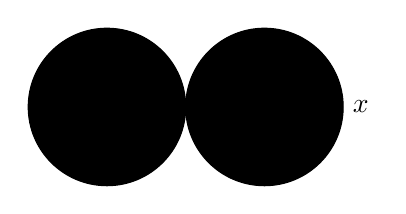
\begin{tikzpicture}
      \draw[->] (-2, 0) -- (2, 0) node[right] {$x$};
      \filldraw (1, 0) circle (\pointSize) node[below] {$1$};
      \filldraw (-1, 0) circle (\pointSize) node[below] {$-1$};
   \end{tikzpicture}
   \caption{Đồ thị phần 1 bài \ref{intropt}}
   \label{fig:dtp1}
\end{wrapfigure}

Giải phương trình:
\begin{align*}
   &x^2 - 1 = 0 \\
   \iff &x^2 = 1 \\
   \iff &x \in \{-1; 1\}
\end{align*}
và từ đó, đồ thị của $\mathcal{P}$ có được như hình \ref{fig:dtp1}.
}

\begin{wrapfigure}{R}{0.5\textwidth}
   \centering
   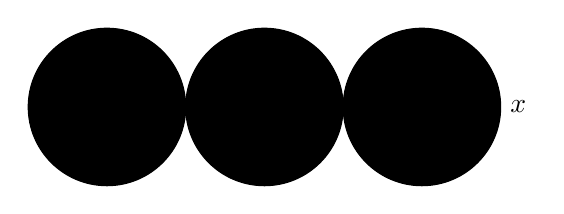
\begin{tikzpicture}
      \draw[->] (-2, 0) -- (4, 0) node[right] {$x$};
      \filldraw (1, 0) circle (\pointSize) node[below] {$1$};
      \filldraw (-1, 0) circle (\pointSize) node[below] {$-1$};
      \filldraw (3, 0) circle (\pointSize) node[below] {$3$};
      
   \end{tikzpicture}
   \caption{Đồ thị phần 2 bài \ref{intropt}}
   \label{fig:dtp2}
\end{wrapfigure}
2. $\mathcal{P}$ là phương trình chỉ có một ẩn $x$, do đó đồ thị của $\mathcal{P}$ chỉ là đồ thị một chiều trên một trục số biểu diễn cho $x$. 

Có ba giá trị để $f(x)$ bằng $0$: $x\in \{-1; 1; -3\}$. Chúng ta có đồ thị của $\mathcal{P}$ ở hình \ref{fig:dtp2}.

3. Tập xác định của $f(x)$ là $\{-1; 1; -2; 2; -3; 3\}$, do đó, để $\mathcal{P}$ thỏa mãn thì $x$ chí có thể nhận các giá trị trong vùng tập xác định.

{
\begin{wrapfigure}{R}{0.5\textwidth}
   \centering
   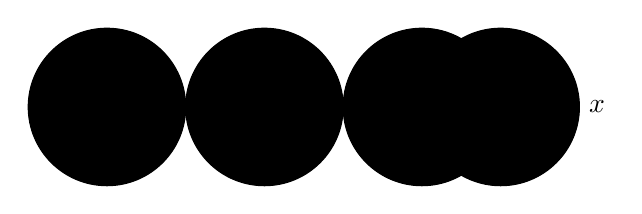
\begin{tikzpicture}
      \draw[->] (-4, 0) -- (3, 0) node[right] {$x$};
      \filldraw (1, 0) circle (\pointSize) node[below] {$1$};
      \filldraw (-1, 0) circle (\pointSize) node[below] {$-1$};
      \filldraw (-3, 0) circle (\pointSize) node[below] {$-3$};
      \filldraw (2, 0) circle (\pointSize) node[below] {$2$};
   \end{tikzpicture}
   \caption{Đồ thị phần 3 bài \ref{intropt}}
   \label{fig:dtp3}
\end{wrapfigure}
Kẻ bảng so sánh:
   
\begin{table}[h]
   \begin{minipage}{0.5\textwidth}
      \centering
         \begin{tabular}{|c|c|c|c|c|c|c|}
            \hline
            $x$ & $-1$ & $1$ & $-2$ & $2$ & $-3$ & $3$\\
            \hline
            $f(x)$ & $0$ & $0$ & $4$ & $3$ & $7$ & $0$\\
            \hline
            $x^2-1$ & $0$ & $0$ & $3$ & $3$ & $7$ & $7$\\
            \hline
         \end{tabular}
         \caption{Giá trị của $f(x)$ và $x^2-1$ ứng với $x$}
         \label{tab:values3}
   \end{minipage}
\end{table}

\noindent Nhận thấy rằng $\mathcal{P}$ chỉ đúng khi $x\in \{-1; 1; -3; 2\}$ và chúng ta có đồ thị là hình \ref{fig:dtp3}.
}

\begin{wrapfigure}{R}{0.5\textwidth}
   \centering
   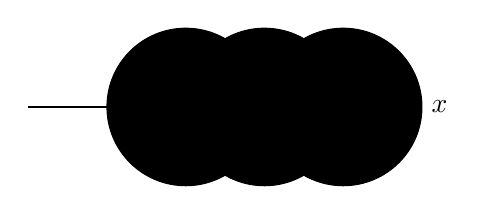
\begin{tikzpicture}
      \draw[->] (0, 0) -- (5, 0) node[right] {$x$};
      \filldraw (2, 0) circle (\pointSize) node[below] {$2$};
      \filldraw (3, 0) circle (\pointSize) node[below] {$3$};
      \filldraw (4, 0) circle (\pointSize) node[below] {$4$};
      
   \end{tikzpicture}
   \caption{Đồ thị phần 4 bài \ref{intropt}}
   \label{fig:dtp4}
\end{wrapfigure}
4. Nhìn vào bảng được cho, có $f(x) = g(x)$ khi và chỉ khi $x\in \{2; 3; 4\}$. Do đó, đồ thị của $\mathcal{P}$ có được như hình \ref{fig:dtp4}.

5. $\mathcal{P}$ là phương trình có hai ẩn $x$ và $y$, do đó đồ thị của $\mathcal{P}$ là một mặt phẳng hai chiều. Coi như trục hoành biểu diễn cho $x$ và trục tung biểu diễn cho $y$. 

\begin{wraptable}{R}{0.5\textwidth}
   \centering
   \begin{tabular}{|c|c|c|c|c|}
      \hline
      $B_n$ & $3$ & $5$ & $7$ & $11$ \\
      \hline
      $x$ & $2$ & $3$ & $4$ & $5$ \\
      \hline
      $y$ & $2$ & $3$ & $4$ & $6$ \\
      \hline 
   \end{tabular}
   \caption{Giá trị của $x$ và $y$ ứng với $B_n$}
   \label{tab:bn_values}
\end{wraptable}

Để có thể vẽ được đồ thị của $\mathcal{P}$, hiển nhiên nhìn ra được rằng cần phải có những điểm $(x;y)$ để hai giá trị $f(x)$ và $g(y)$ bằng nhau. Và để làm được điều đó, trước hết, chúng ta sẽ tìm xem giá trị bằng nhau của $f(x)$ với $g(y)$ này bằng bao nhiêu. Gọi chung giá trị bằng nhau này là $B_n$. Kẻ lại bảng so sánh thành bảng \ref{tab:bn_values}, với $B_n$ là ra trị đầu ra và $x$, $y$ là giá trị lần lượt đưa vào hai hàm $f$ và $g$ để có giá trị đầu ra đó. Và từ đó, chúng ta có đồ thị của $\mathcal{P}$ là hình \ref{fig:dtp5}.

\begin{figure}[h]
   \centering
   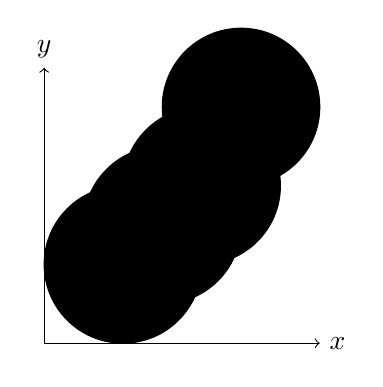
\begin{tikzpicture}
      \draw[->] (0, 0) -- (3.5, 0) node[right] {$x$};
      \draw[->] (0, 0) -- (0, 3.5) node[above] {$y$};
      \filldraw (1, 1) circle (\pointSize) node[right] {$(2; 2)$};
      \filldraw (1.5, 1.5) circle (\pointSize) node[right] {$(3; 3)$};
      \filldraw (2.5, 3) circle (\pointSize) node[right] {$(5; 6)$};
      \filldraw (2, 2) circle (\pointSize) node[right] {$(4; 4)$};
   \end{tikzpicture}
   \caption{Đồ thị phần 5 bài \ref{intropt}}
   \label{fig:dtp5}
\end{figure}

6. $\mathcal{P}$ là phương trình có hai ẩn $x$ và $b$, do đó đồ thị của $\mathcal{P}$ là một mặt phẳng hai chiều. Coi như trục hoành biểu diễn cho $x$ và trục tung biểu diễn cho $b$.

Giải ngược $b$ từ $f(x)$:
\begin{align*}
   f(x) &= 2b - 1 \\
   \iff b &= \frac{f(x) + 1}{2}.
\end{align*}

Từ đây, chúng ta có thể thêm giá trị của $b$ vào bảng được cho thành bảng \ref{tab:b_values6}

\begin{table}[h]
   \centering
   \begin{tabular}{|c|c|c|c|c|c|c|}
      \hline
      $x$ & $1$ & $2$ & $3$ & $4$ & $5$ & $6$\\
      \hline
      $f(x)$ & $2$ & $3$ & $5$ & $7$ & $11$ & $13$\\
      \hline
      $b$ & $\frac{3}{2}$ & $\frac{5}{2}$ & $3$ & $4$ & $6$ & $7$\\
      \hline
   \end{tabular}
   \caption{Giá trị của $b$ ứng với $x$}
   \label{tab:b_values6}
\end{table}

Qua bảng đó, vẽ được đồ thị của $\mathcal{P}$ như hình \ref{fig:dtp6}.

\begin{figure}[h]
   \centering
   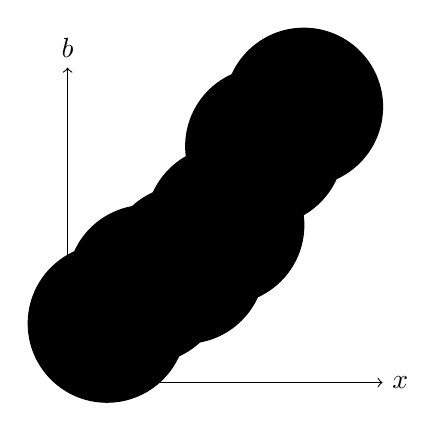
\begin{tikzpicture}
      \draw[->] (0, 0) -- (4, 0) node[right] {$x$};
      \draw[->] (0, 0) -- (0, 4) node[above] {$b$};
      \filldraw (0.5, 0.75) circle (\pointSize) node[below] {$\left(1; \frac{3}{2}\right)$};
      \filldraw (1, 1.25) circle (\pointSize) node[below] {$\left(2; \frac{5}{2}\right)$};
      \filldraw (1.5, 1.5) circle (\pointSize) node[right] {$(3; 3)$};
      \filldraw (2, 2) circle (\pointSize) node[right] {$(4; 4)$};
      \filldraw (2.5, 3) circle (\pointSize) node[right] {$(5; 6)$};
      \filldraw (3, 3.5) circle (\pointSize) node[right] {$(6; 7)$};
   \end{tikzpicture}
   \caption{Đồ thị phần 6 bài \ref{intropt}}
   \label{fig:dtp6}
\end{figure}

7. Nhìn vào bảng, $f(x)$ có thể nhận các giá trị là $\{0; 3; 4; 7\}$.

Khi $f(x) \neq 0$, chỉ có một giá trị đầu vào cho $f$ sao cho $f(x)$ đạt được giá trị đầu ra. Ví dụ, chỉ có đầu vào $x = 2$ mới có $f(x) = 3$. Do đó, khi $f(x) \neq 0$, $x = 2b-1$. Biến đổi đại số cơ bản để có $b = \frac{x + 1}{2}$. Kẻ bảng:

\begin{table}[h]
   \centering
   \begin{tabular}{|c|c|c|c|}
      \hline
      $x$ & $-2$ & $2$ & $-3$\\
      \hline
      $b = \frac{x+1}{2}$ & $-\frac{3}{2}$ & $2$ & $-1$\\
      \hline
   \end{tabular}
   \caption{Giá trị của cặp $(x; b)$ với $f(x) \neq 0$}
   \label{tab:b_values7}
\end{table}

Khi $f(x) = 0$, $x$ và $2b-1$ có thể nhận bất cứ giá trị nào trong tập $\{-1; 1; -3\}$. Từ đó, có thể chọn $x \in \{-1; 1; 3\}$ và giải đại số để chọn $b \in \left\{\frac{-1+1}{2}; \frac{1+1}{2}; \frac{3+1}{2}\right\} = \{0; 1; 2\}$. Các cặp $(x; b)$ thỏa mãn là $(x; b) \in \left\{\left(-1; 0\right); \left(-1; 1\right); \left(-1; 2\right); \left(1; 0\right); \left(1; 1\right); \left(1; 2\right); \left(-3; 0\right); \left(-3; 1\right); \left(-3; 2\right)\right\}$.

Cuối cùng, kết hợp hai trường hợp, chúng ta có đồ thị cho $\mathcal{P}$:

\begin{figure}[H]
   \centering
   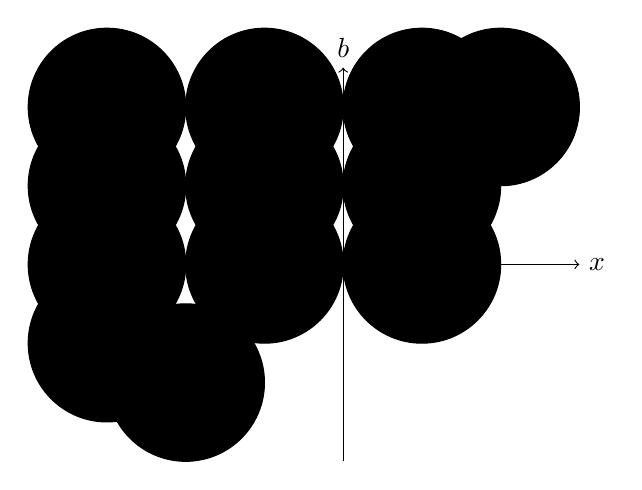
\begin{tikzpicture}
      \draw[->] (-4, 0) -- (3, 0) node[right] {$x$};
      \draw[->] (0, -2.5) -- (0, 2.5) node[above] {$b$};
      
      % Vẽ phần f(x) khác 0
      \filldraw (-2, -1.5) circle (\pointSize) node[below] {$\left(-2; -\frac{3}{2}\right)$};
      \filldraw (2, 2) circle (\pointSize) node[below] {$\left(2; 2\right)$};
      \filldraw (-3, -1) circle (\pointSize) node[below] {$\left(-3; -1\right)$};

      \filldraw (-1, 0) circle (\pointSize) node[below] {$\left(-1; 0\right)$};
      \filldraw (1, 0) circle (\pointSize) node[below] {$\left(1; 0\right)$};
      \filldraw (-3, 0) circle (\pointSize) node[below] {$\left(-3; 0\right)$};

      \filldraw (-1, 1) circle (\pointSize) node[below] {$\left(-1; 1\right)$};
      \filldraw (1, 1) circle (\pointSize) node[below] {$\left(1; 1\right)$};
      \filldraw (-3, 1) circle (\pointSize) node[below] {$\left(-3; 1\right)$};

      \filldraw (-1, 2) circle (\pointSize) node[below] {$\left(-1; 2\right)$};
      \filldraw (1, 2) circle (\pointSize) node[below] {$\left(1; 2\right)$};
      \filldraw (-3, 2) circle (\pointSize) node[below] {$\left(-3; 2\right)$};
   \end{tikzpicture}
   \caption{Đồ thị phần 7 bài \ref{intropt}}
   \label{fig:dtp7}
\end{figure}

8. $\mathcal{P}$ là phương trình có ba ẩn $a$, $b$ và $c$, do đó đồ thị của $\mathcal{P}$ là một mặt phẳng ba chiều. Coi như trục hoành biểu diễn cho $a$, trục tung biểu diễn cho $b$ và trục cao biểu diễn cho $c$.

Theo $\mathcal{P}$, chúng ta cần phải chọn ba số trong tập giá trị của $f$ để hai trong ba số có tổng bằng số còn lại. Từ bảng, nhận thấy rằng, chỉ có thể có hai tổng $4 + 3 = 7$ và $0 + 0 = 0$.

Xét trường hợp đầu tiên, chúng ta có $f(c) = 7$ và $\left(f(a); f(b)\right) \in \left\{\left(4; 3\right); \left(3; 4\right)\right\}$. Tìm ngược lại đầu vào để được $(a; b; c) \in \left\{\left(2; -2; -3\right); \left(-2; 2; -3\right)\right\}$.

Xét trường hợp thứ hai, chúng ta có $f(a) = f(b) = f(c) = 0$. Từ đó, $a$, $b$ và $c$ có thể nhận bất cứ giá trị nào trong tập $\{-3; -1; 1\}$.

Kết hợp hai trường hợp, đồ thị cuối cùng của $\mathcal{P}$ sẽ là hình \ref{fig:dtp8}.

\begin{figure}[H]
   \centering
   \tdplotsetmaincoords{80}{30}
   \begin{tikzpicture}[tdplot_main_coords]
      \draw[->] (-5, 0, 0) -- (2, 0, 0) node[right] {$a$};
      \draw[->] (0, -5, 0) -- (0, 4, 0) node[above] {$b$};
      \draw[->] (0, 0, -4) -- (0, 0, 2) node[above] {$c$};
      \filldraw (2, -2, -3) circle (\pointSize) node[font=\scriptsize, anchor=north] {$\left(2; -2; -3\right)$};  
      \filldraw (-2, 2, -3) circle (\pointSize) node[font=\scriptsize, anchor=south] {$\left(-2; 2; -3\right)$};  
      \foreach \x/\y/\z in {
         -3/-3/-3, -3/-3/-1, -3/-3/1, 
         -3/-1/-3, -3/-1/-1, -3/-1/1, -3/1/-3, -3/1/-1, -3/1/1,
         -1/-3/-3, -1/-3/-1, -1/-3/1, -1/-1/-3, -1/-1/-1, -1/-1/1,
         -1/1/-3, -1/1/-1, -1/1/1, 1/-3/-3, 1/-3/-1, 1/-3/1,
         1/-1/-3, 1/-1/-1, 1/-1/1, 1/1/-3, 1/1/-1, 1/1/1
      } {
         \filldraw (\x, \y, \z) circle (\pointSize);
         \node[font=\scriptsize, anchor=east] at (\x, \y, \z) {$\left(\x, \y, \z\right)$};
      }

   \end{tikzpicture}
   \caption{Đồ thị phần 8 bài \ref{intropt}}
   \label{fig:dtp8}
\end{figure}

\exercise[ex:hpt1] Vẽ đồ thị của hệ phương trình $\mathcal{P}$, với các định nghĩa đã cho. Hàm có tập xác định là bộ số đầu vào cho ở trong bảng.
\begin{enumerate}
   \item 
   \begin{tabular}{|c|c|c|c|c|c|c|}
      \hline
      $x$ & $0$ & $1$ & $2$ & $3$ & $4$ & $5$ \\
      \hline
      $f(x)$ & $-1$ & $-1$ & $-1$ & $-2$ & $-3$ & $-3$\\
      \hline
   \end{tabular},
   \begin{tabular}{|c|c|c|c|c|c|c|}
      \hline
      $y$ & $0$ & $-2$ & $4$ & $-6$ & $8$ & $-10$\\
      \hline
      $g(y)$ & $-1$ & $-2$ & $-3$ & $-7$ & $-8$ & $-9$\\
      \hline
   \end{tabular},

   \noindent\begin{tabular}{|c|c|c|c|c|c|c|}
      \hline
      $z$ & $-1$ & $1$ & $-2$ & $0$ & $-4$ & $4$\\
      \hline
      $h(z)$ & $2$ & $1$ & $0$ & $-1$ & $-2$ & $-3$\\
      \hline
   \end{tabular} và $\mathcal{P}:f(x) = g(x) = h(x)$;

   \item
   \begin{tabular}{|c|c|c|c|c|c|c|}
      \hline
      $x$ & $0$ & $1$ & $2$ & $3$ & $4$ & $5$ \\
      \hline
      $f(x)$ & $-1$ & $-1$ & $-1$ & $-2$ & $-3$ & $-3$\\
      \hline
   \end{tabular},
   \begin{tabular}{|c|c|c|c|c|c|c|}
      \hline
      $y$ & $0$ & $-2$ & $4$ & $-6$ & $8$ & $-10$\\
      \hline
      $g(y)$ & $-1$ & $-2$ & $-3$ & $-7$ & $-8$ & $-9$\\
      \hline
   \end{tabular},

   \noindent\begin{tabular}{|c|c|c|c|c|c|c|}
      \hline
      $z$ & $-1$ & $1$ & $-2$ & $0$ & $-4$ & $4$\\
      \hline
      $h(z)$ & $2$ & $1$ & $0$ & $-1$ & $-2$ & $-3$\\
      \hline
   \end{tabular} và $\mathcal{P}:f(a) = g(b) = h(c)$;

   \item
   \begin{tabular}{|c|c|c|c|c|c|c|}
      \hline
      $x$ & $0$ & $1$ & $2$ & $3$ & $4$ & $5$ \\
      \hline
      $f(x)$ & $-1$ & $-1$ & $-1$ & $-2$ & $-3$ & $-3$\\
      \hline
   \end{tabular},
   \begin{tabular}{|c|c|c|c|c|c|c|}
      \hline
      $y$ & $0$ & $-2$ & $4$ & $-6$ & $8$ & $-10$\\
      \hline
      $g(y)$ & $-1$ & $-2$ & $-3$ & $-7$ & $-8$ & $-9$\\
      \hline
   \end{tabular},

   \noindent\begin{tabular}{|c|c|c|c|c|c|c|}
      \hline
      $z$ & $-1$ & $1$ & $-2$ & $0$ & $-4$ & $4$\\
      \hline
      $h(z)$ & $2$ & $1$ & $0$ & $-1$ & $-2$ & $-3$\\
      \hline
   \end{tabular} và $\mathcal{P}:\begin{cases}f(o) = g(p)\\f(p + 1) = h(q)\end{cases}$.

   \item
   \begin{tabular}{|c|c|c|c|c|c|c|}
      \hline
      $x$ & $0$ & $1$ & $2$ & $3$ & $4$ & $5$ \\
      \hline
      $f(x)$ & $-1$ & $-1$ & $-1$ & $-2$ & $-3$ & $-3$\\
      \hline
   \end{tabular},
   \begin{tabular}{|c|c|c|c|c|c|c|}
      \hline
      $y$ & $0$ & $-2$ & $4$ & $-6$ & $8$ & $-10$\\
      \hline
      $g(y)$ & $-1$ & $-2$ & $-3$ & $-7$ & $-8$ & $-9$\\
      \hline
   \end{tabular},

   \noindent\begin{tabular}{|c|c|c|c|c|c|c|}
      \hline
      $z$ & $-1$ & $1$ & $-2$ & $0$ & $-4$ & $4$\\
      \hline
      $h(z)$ & $2$ & $1$ & $0$ & $-1$ & $-2$ & $-3$\\
      \hline
   \end{tabular} và $\mathcal{P}:\begin{cases}f(m) = n\\g(n) = h(w)\end{cases}$.
\end{enumerate}

\solution[ex:hpt1]

\begin{wrapfigure}{R}{0.5\textwidth}
   \centering
   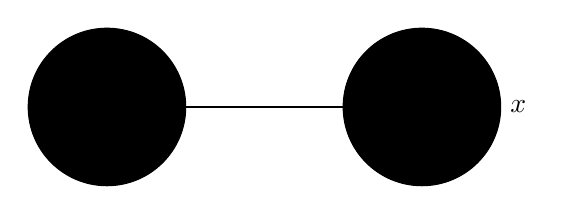
\begin{tikzpicture}
      \draw[->] (-1, 0) -- (5, 0) node[right] {$x$};
      \filldraw (0, 0) circle (\pointSize) node[below] {$0$};
      \filldraw (4, 0) circle (\pointSize) node[below] {$4$};
   \end{tikzpicture}
   \caption{Đồ thị phần 1 bài \ref{ex:hpt1}}
   \label{fig:hpt11}
\end{wrapfigure}

1. Giá trị đầu vào để $f, g, h$ đều có cùng một đầu ra là $x\in\{0;4\}$. Vậy, chúng ta có đồ thị như hình \ref{fig:hpt11}.

2. Trước hết, cần tìm những giá trị chung trong tập giá trị của $f, g, h$. Nhận thấy rằng, có $-1, -2$ và $-3$ là những giá trị chung trong đó. 

\def \hptFntsize {\scriptsize}

\begin{wrapfigure}{L}{0.4\textwidth}
   \centering
   \tdplotsetmaincoords{80}{-10}
   \begin{tikzpicture}[tdplot_main_coords]
      \draw[->] (-1.5, 0, 0) -- (3, 0, 0) node[right] {$a$};
      \draw[->] (0, -1, 0) -- (0, 2.5, 0) node[above] {$b$};
      \draw[->] (0, 0, -2.5) -- (0, 0, 2.5) node[above] {$c$};
      \filldraw (0, 0, 0) circle (\pointSize) node[below left,font=\hptFntsize] {$\left(0; 0; 0\right)$};
      \filldraw (0.5, 0, 0) circle (\pointSize) node[above,font=\hptFntsize] {$\left(1; 0; 0\right)$};
      \filldraw (1, 0, 0) circle (\pointSize) node[below,font=\hptFntsize] {$\left(2; 0; 0\right)$};
      \filldraw (1.5, -1, -2) circle (\pointSize) node[above,font=\hptFntsize] {$\left(3; -2; -4\right)$};
      \filldraw (2, 1, 1) circle (\pointSize) node[above,font=\hptFntsize] {$\left(4; 4; 4\right)$};
      \filldraw (2.5, 1, 1) circle (\pointSize) node[below,font=\hptFntsize] {$\left(5; 4; 4\right)$};
   \end{tikzpicture}
   \caption{Đồ thị phần 2 bài \ref{ex:hpt1}}
   \label{fig:hpt12}
\end{wrapfigure}

Với đầu ra là $-1$, chúng ta có $f(a) = g(b) = h(c) = -1$. Từ đó, chúng ta có
$$
\begin{cases}
   a \in \{0; 1; 2\}\\
   b = 0\\
   c = 0
\end{cases}.
$$ 

Trong trường hợp kết quả của hàm là $-2$, $f(a) = g(b) = h(c) = -2$. Từ đó,
$$
\begin{cases}
   a = 3\\
   b = -2\\
   c = -4
\end{cases}.
$$

Trong trường hợp kết quả của hàm là $-3$, $f(a) = g(b) = h(c) = -3$. Từ đó,
$$
\begin{cases}
   a \in \{4; 5\}\\
   b = 4\\
   c = 4
\end{cases}.
$$

Kết hợp ba trường hợp, xây dựng không gian tọa độ, chúng ta có hình \ref{fig:hpt12}.

3. Để $f$ và $g$ nhận cùng một giá trị thì giá trị đầu ra đó, theo bảng, phải là $-1$, $-2$ hoặc $-3$.

\begin{wrapfigure}{L}{0.4\textwidth}
   \tdplotsetmaincoords{80}{-10}
   \centering
   \begin{tikzpicture}[scale=0.5, tdplot_main_coords]
      \draw[->] (-2, 0, 0) -- (6, 0, 0) node[right] {$o$};
      \draw[->] (0, -2, 0) -- (0, 5, 0) node[above] {$p$};
      \draw[->] (0, 0, -2) -- (0, 0, 5) node[above] {$q$};
      \filldraw (0, 0, 0) circle (\pointSize * 2) node[below left,font=\hptFntsize] {$\left(0; 0; 0\right)$};
      \filldraw (1, 0, 0) circle (\pointSize * 2) node[above,font=\hptFntsize] {$\left(1; 0; 0\right)$};
      \filldraw (2, 0, 0) circle (\pointSize * 2) node[below,font=\hptFntsize] {$\left(2; 0; 0\right)$};
      \filldraw (4, 4, 4) circle (\pointSize * 2) node[above,font=\hptFntsize] {$\left(4; 4; 4\right)$};
      \filldraw (5, 4, 4) circle (\pointSize * 2) node[below,font=\hptFntsize] {$\left(5; 4; 4\right)$};
   \end{tikzpicture}
   \caption{Đồ thị phần 3 bài \ref{ex:hpt1}}
   \label{fig:hpt13}
\end{wrapfigure}

Tại $f(o) = g(p) = -1$, $o \in \{0; 1; 2\}$ và $p = 0$. Từ đó, $f(p + 1) = f(1) = -1$. Khi này, $h(q) = -1 \iff q = 0$.

Tại $f(o) = g(p) = -2$, sau khi tra bảng, chúng ta thấy được rằng $\begin{cases}o = 3\\p = -2\end{cases}$; suy ra $f(p + 1) = f(-1)$. Tuy nhiên, $-1$ không thuộc tập xác định của $f$. Vậy, chúng ta sẽ loại trường hợp này.

Tại $f(o) = g(p) = -3$, $o \in \{4; 5\}$ và $p = 4$. Từ đó, $f(p + 1) = f(5) = -3$. Khi này, $h(q) = -3 \iff q = 4$.

Cuối cùng, vẽ đồ thị để được hình \ref{fig:hpt13}.

\begin{wrapfigure}{L}{0.4\textwidth}
   \tdplotsetmaincoords{80}{20}
   \centering
   \begin{tikzpicture}[scale=0.5, tdplot_main_coords]
      \draw[->] (-1, 0, 0) -- (4, 0, 0) node[right] {$o$};
      \draw[->] (0, -3, 0) -- (0, 1, 0) node[above] {$p$};
      \draw[->] (0, 0, -5) -- (0, 0, 1) node[above] {$q$};
      \filldraw (3, -2, -4) circle (\pointSize * 2) node[above,font=\hptFntsize] {$\left(3; -2; -4\right)$};
   \end{tikzpicture}
   \caption{Đồ thị phần 4 bài \ref{ex:hpt1}}
   \label{fig:hpt14}
\end{wrapfigure}

4. Theo đề, chúng ta cần tìm những bộ $(m;n;w)$ thỏa mãn $\mathcal{P}$, trong đó có $g(n) = h(w)$. Cho nên, $n$ phải thuộc tập xác định của $g$. Nhìn vào bảng, tập xác định đó là $\{0; -2; 4; -6; 8; -10\}$. Tuy nhiên, cũng có $f(m) = n$, cho nên $n$ vừa phải thuộc tập giá trị của $f$, hay $n \in \{-1; -2; -3\}$. Lấy giao của hai tập đó, chúng ta có $n = -2$. Từ đó, giải $f(m) = -2$ để có $m = 3$. Thêm vào đó, $h(w) = g(-2) = -2 \iff w = -4$.

Bộ số duy nhất thỏa mãn hệ phương trình $\mathcal{P}$ là $\left(m; n; w\right) = \left(3; -2; -4\right)$. Đồ thị của $\mathcal{P}$ là hình \ref{fig:hpt14}.